\begin{center}
    % Gain
    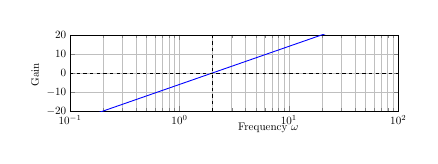
\begin{tikzpicture}
        [
            scale = 0.4,
            >=latex
        ]
        \begin{axis}
            [
                width=12cm,
                height=4cm,
                xmode=log,
                xmin=0.1, xmax=100, ymin=-20, ymax=20,
                x label style={anchor=west},
                xlabel=Frequency $\omega$,
                y label style={anchor=south},
                ylabel=Gain $\deci \bel$,
                xmajorgrids=true,
                xminorgrids=true,
                ymajorgrids=true
            ]

            \addplot[thick, color=blue, domain=0.1:100]{20*log10(x)-6};

            \addplot[dashed, color=black, domain=0.1:100]{0};
            \addplot[dashed, color=black, domain=2:2] coordinates {(2, -20) (2, 20)};
        \end{axis}
        
    \end{tikzpicture}


    % Phase
    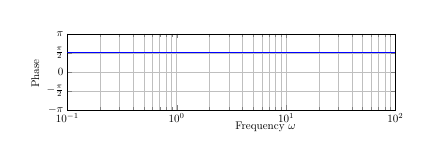
\begin{tikzpicture}
        [
            scale = 0.4,
            >=latex
        ]
        \begin{axis}
            [
                width=12cm,
                height=4cm,
                xmode=log,
                xmin=0.1, xmax=100, ymin=-3.141, ymax=3.141,
                x label style={anchor=west},
                xlabel=Frequency $\omega$,
                y label style={anchor=south},
                ylabel=Phase $\rad$,
                ytick={-3.14, -1.57, 0, 1.57, 3.14},
                yticklabels={$-\pi$, $-\frac{\pi}{2}$, $0$, $\frac{\pi}{2}$, $\pi$},
                xmajorgrids=true,
                xminorgrids=true,
                ymajorgrids=true
            ]
            
            \addplot[thick, color=blue, domain=0.1:100]{1.57};                 
        \end{axis}
            
    \end{tikzpicture}
\end{center}

